\documentclass{../oss-apphys-exam}

\begin{document}
\gentitle{10}{PHYSICS OF SOUND AND MUSIC}

\begin{questions}
  \question Beats are the result of:
  \begin{choices}
    \choice diffraction
    \choice constructive interference
    \choice destructive interference
    \choice both constructive and destructive interference
  \end{choices}

  \question Sound waves are:
  \begin{choices}
    \choice longitudinal
    \choice transverse
    \choice partly longitudinal and partly transverse
    \choice torsional
  \end{choices}

  \question The intensity of a sound at \SI{200}{\metre} is
  \underline{\hspace{1in}} the intensity of sound at \SI{100}\metre.
  \begin{choices}
  \item 2 times
  \item 4 times
  \item $1/2$ times
  \item $1/4$ times
  \item the same as
  \end{choices}
  
  \question Sound travels fastest in:
  \begin{choices}
    \choice cool air
    \choice water
    \choice warm air
    \choice vacuum
  \end{choices}

  %\question Sound waves do not travel through:
  %  \begin{choices}
  %  \item solids
  %  \item gases
  %  \item liquids
  %  \item a vacuum
  %  \end{choices}
  
  %\question Harmonics are resonance modes that are also called:
  %  \begin{choices}
  %  \item pitch
  %  \item loudness
  %  \item overtones
  %  \item resonance
  %  \end{choices}

  \question The intensity of a sound wave refers to its:
  \begin{choices}
    \choice pitch
    \choice loudness
    \choice overtones
    \choice resonance
  \end{choices}

  %\question A pure musical tone causes a thin wooden panel to vibrate. This is
  %an example of:
  %\begin{choices}
  %  \choice an overtone
  %  \choice harmonics
  %  \choice resonance
  %  \choice interference
  %\end{choices}
  
  \question A loud boom is heard after an airplane has passed overhead. This
  means that the airplane:
  \begin{choices}
    \choice is accelerating
    \choice is climbing
    \choice is travelling faster than Mach 1
    \choice is travelling faster than the speed of light
  \end{choices}
  
  \question A spacecraft speeding away from Earth sends out signals of a certain
  frequency. The signals that are received on the Earth
  \begin{choices}
    \choice have a lower speed
    \choice have extra harmonics
    \choice have a longer wavelength
    \choice have all of the above characteristics
  \end{choices}
  \newpage
  
  \question Two tuning forks of frequencies \num{310} and \SI{316}{\hertz}
  vibrate simultaneously. The number of times the resulting sound pulsates per
  second is:
  \begin{choices}
    \choice 0
    \choice 6
    \choice 313
    \choice 626
  \end{choices}

  %\question An octave ``up'' in music involves \underline{\hspace{1in}}
  %the frequency. %(Google if you didn't understand it in class.)
  %\begin{choices}
  %  \choice slightly increasing
  %  \choice doubling
  %  \choice tripling
  %  \choice slightly decreasing
  %\end{choices}

  \question A guitar player plays a \SI{440}{\hertz} note, and then increases
  the effective length of that same guitar string by a factor of two and plays
  it again. The new frequency is:
  \begin{choices}
    \choice \SI{440}\hertz
    \choice \SI{880}\hertz
    \choice \SI{220}\hertz
    \choice \SI0\hertz
  \end{choices}

  \question The purpose of the intricately shaped and delicately made violin
  wooden body is to
  \begin{choices}
    \choice hold the strings tight
    \choice amplify the string vibration
    \choice look impressive
    \choice strengthen the wood
  \end{choices}
  
  \question A flute can be tuned to the rest of the orchestra by adjusting its
  length. A flute player is playing on a very hot day and wishes to play the
  proper frequencies. Compared to the length in the cooler practice hall, the
  length of the flute must be:
  \begin{choices}
    \choice slightly greater
    \choice slightly less
    \choice a lot less
    \choice unchanged
  \end{choices}

  \question A dust particle is suspended in air (floating due to a small updraft
  and its own low mass) when a powerful loudspeaker emits a low frequency
  of \SI{2}\hertz. (This frequency cannot be heard but you can actually see
  the speaker move). How will the dust particle move as a result of the speaker
  being turned on?
  
  \begin{minipage}{.6\textwidth}
    \begin{choices}
    \item The dust particle will move up and down
    \item The dust particle will be pushed across the room
    \item The dust particle will move side to side
    \item The dust particle will move in a circular path
    \end{choices}
  \end{minipage}
  \begin{minipage}{.3\textwidth}
    \begin{center}
      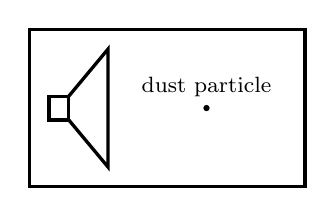
\begin{tikzpicture}[scale=.5,very thick]
        \draw (0,0) rectangle (7,4);
        \draw (.5,1.7) rectangle (1,2.3);
        \draw (1,1.7)--(2,.5)--(2,3.5)--(1,2.3);
        \fill (4.5,2) circle (.08) node[above]{\footnotesize dust particle};
      \end{tikzpicture}
    \end{center}
  \end{minipage}
  
  %\question Fill in the blanks:
  %\begin{parts}
  %  \part Vibrations at an angle of \ang{90} to the direction of propagation
  %  are \underline{\hspace{1.5in}} waves.
  %  
  %  \part Sounds above the sonic frequency range of humans are known as
  %  \underline{\hspace{1in}} and below the sonic frequency range the sound are
  %  called \underline{\hspace{1in}}.
  %
  %  \part The number of cycles per second a sound wave delivers to the ear is
  %  its \underline{\hspace{1in}} to a physicist but musicians or the general
  %  public refer to this as \underline{\hspace{1in}}.
  %\end{parts}

  %\question An oscilloscope is used to record the sounds made by four students.
  %The equally scaled wave-forms are shown below:
  %\begin{center}
  %  \vspace{-.1in}
  %  \begin{tikzpicture}[scale=.65]
  %    \draw (2,0) circle (2);
  %    \node[below] at (2,-2) {Alex};
  %    \draw[smooth,samples=35,domain=0:3.96,thick] plot(\x,{.18*sin(200*\x)});
  %  \end{tikzpicture}
  %  \begin{tikzpicture}[scale=.65]
  %    \draw (2,0) circle (2);
  %    \node[below] at (2,-2) {Brenda};
  %    \draw[smooth,samples=50,domain=0:3.85,thick] plot(\x,{.8*sin(350*\x)});
  %  \end{tikzpicture}
  %  \begin{tikzpicture}[scale=.65]
  %    \draw (2,0) circle (2);
  %    \node[below] at (2,-2) {Celia};
  %    \draw[smooth,samples=40,domain=0:3.945,thick] plot(\x,{.4*sin(150*\x)});
  %  \end{tikzpicture}
  %  \begin{tikzpicture}[scale=.65]
  %    \draw (2,0) circle (2);
  %    \node[below] at (2,-2) {Doug};
  %    \draw[smooth,samples=20,domain=0:3.9,thick] plot(\x,{1.2*sin(100*\x)});
  %  \end{tikzpicture}
  %\end{center}
  %\begin{enumerate}[itemsep=.15in,label=(\alph*)]
  %\item Which sound is the softest? \underline{\hspace{1in}}
  %\item Which sound has the highest frequency? \underline{\hspace{1in}}
  %\item Which sound has the longest wavelength? \underline{\hspace{1in}}
  %\item Which sound shows about $1\dfrac12$ cycles? \underline{\hspace{1in}}
  %%\item Which person has the highest voice? \underline{\hspace{1in}}
  %\end{enumerate}

%\item Researchers interested in global warming can release sound waves that
%  travel underwater to detection devices located around the planet. Explain how
%  this works in terms of the physics of sound. Some questions to consider:
%  \begin{itemize}
%  \item How does this help them determine the temperature of the ocean?
%  \item What property of waves do they utilize and how does this property
%    change as it travels through different parts of the world's oceans?
%  \item If the ocean was really warming up how would their observations at the
%    detectors change?
%  \end{itemize}
%  \vspace{2in}

%  \item the actual particles in a sound wave travelling in an open tube and
%    indicate the wavelength and regions of low density air, normal density air,
%    and high density air. Explain how this can be represented by a sin wave.
%  \end{enumerate}
%\end{enumerate}

  \question When a violin string is played without fingering simultaneously
  with a tuning fork of frequency \SI{440}\hertz, beats are heard at a rate
  of 3 per second. When the tension in the string is increased slightly, the
  beat frequency decreases. What was the initial frequency of the violin string?
  \newpage
  
  \question A jet is travelling at Mach number of $M=1.6$ at an altitude of
  \SI{8000}\metre.
  \begin{parts}
    \part What is the angle of the shock wave makes with the track of the jet?
    \vspace{\stretch1}
    
    \part Where is the jet when a person on the ground hears the shock wave?
    \vspace{\stretch1}
  \end{parts}
  
  \question You know that the pitch of a train's whistle is about
  \SI{5.0}{\kilo\hertz}. As you stand at a railway crossing, you hear a train
  whistle whose frequency is \SI{6.0}{\kilo\hertz}.
  \begin{parts}
  \item Is the train approaching you or travelling away from you? Explain your
    answer.
  \item If the temperature of that day is a warm \SI{30}\celsius, how fast is
    the train moving?
  \end{parts}
  \vspace{\stretch2}

  \question The G string on a violin is \SI{30}{\centi\metre} long. When played
  without fingering (violinists call it an ``open string''), it vibrates at a
  fundamental frequency of \SI{196}{\hertz}. The next higher note on a G-major
  scale is A (\SI{220}\hertz). %and B (\SI{247}{\hertz}).
  How far from the end of the string must a finger be placed to play that note?
  \vspace{\stretch2}
  \newpage
  
  \question The normal range of hearing of an average adult is about 20 to
  \SI{20000}\hertz.
  \begin{parts}
    \part What is the greatest length of an organ pipe that would have its
    fundamental note in this range if it is closed at one end? Assume a speed
    of sound of \SI{340}{\metre\per\second} at room temperature.
    \vspace{\stretch1}

    \part The shortest pipes in organs are about \SI{7.5}{\centi\metre} long.
    What is the fundamental frequency of a pipe if it is open at both ends?
    \vspace{\stretch1}

    \part For the \SI{7.5}{\centi\metre} organ pipe, what is the highest
    harmonic that is within the audible range?
    \vspace{\stretch1}
  \end{parts}  
  %What are the frequencies if the temperature is raised to \SI{28}\celsius?
  
%  \question A student carefully makes the following observations listening for
%  the resonance points from a tuning fork vibrating above an adjustable length
%  pipe that is open on one end:
%  \begin{itemize}[nosep]
%    \item Temperature is \SI{13.3}\celsius
%    \item First resonant length: $L_1=\SI{8.3}{\centi\metre}$
%  \end{itemize}
%  Then he rushes his following measurements for additional resonance points
%  to finish the lab:
%  \begin{itemize}[nosep]
%  \item Second resonance length $L_2=\SI{25}{\centi\metre}$
%  \item Third resonance length $L_3=\SI{58}{\centi\metre}$
%  \end{itemize}
%  \begin{parts}
%    \part Draw diagrams (waveform inside the pipe) for the first two
%    resonant lengths collected.
%    \part Find the frequency of the unknown tuning fork.
%    \part Analyze all the data to see if he made any errors in their collection
%    of observations. If he has made an error, what is it?
%  \end{parts}

  \question Three successive resonance frequencies in an organ pipe are 1310,
  1834, and \SI{2358}\hertz. Is the pipe closed at one end or open at both
  ends? What is the fundamental frequency? What is the length of the pipe if the
  speed of sound is \SI{340}{\metre\per\second}?
  \vspace{\stretch3}
  
  %\question Describe what you would see when a standing wave was set up in a
  % spring. Why is it called a standing wave?

  %\question What is a node? What is an anti-node? Describe how the nodes and
  %anti-nodes are distributed along the length of the standing wave pattern.

  %\question A skyscraper will often oscillate due to wind blowing against it
  %(gusting). It vibrates like a semi-open pipe in fundamental mode (node at the
  %bottom of the building, anti-node at the top). Engineers calculate that the
  %transverse waves will travel through the structure at a speed of
  %\SI{45}{\meter\per\second}. For a wind that typically gusts with a period of
  %\SI{12.0}\second, what height of the building will vibrate the most?
  %\vspace{\stretch1}
  
  %\question A clarinet behaves like a semi-open pipe with the open end at the
  %bell and closed end at the reed. Claudia blows very gently---just enough to
  %play a low A with a frequency of \SI{220}\hertz. She then blows harder
  %(overblows) using the same fingering and produce the next higher note (the
  %next resonance mode). What is the frequency of the higher note? Can you
  %determine its pitch?

  %\question The sound of a starting pistol can be heard easily from a distance
  %of \SI{800}{\metre} but the smoke can be seen much sooner than the sound is
  %perceived. Why is the smoke seen before the sound is heard? What is the time
  %delay for the sound of the pistol if the air temperature is
  %\SI{15}\celsius?

  %\questions A general rule for finding the distance to a lightning flash is to
  %begin counting when the flash is observed and stop when the thunder clap is
  %heard. The number of seconds counted is then divided by 3 to get the distance
  %in kilometres. Why is this justified? How accurate is this procedure? Is a
  %correction for the time is takes for the light to reach you important? (The
  %speed of light is \SI{3e8}{\metre\per\second}.)
  
  %\question You decide to create a jug and bottle band where you want to play
  %the bottles and jugs by blowing across the tops of the bottles to generate
  %sounds. What is the largest/longest container you will need based on the
  %human range of hearing? What is the shortest? Are these reasonable jug sizes?
  %Illustrate your explanation with a diagram. (Human can hear approximately
  %from \SI{20}{\hertz} to \SI{20000}\hertz.)

  %\question An organ pipe open at one end and closed at the other is
  %\SI{30}{\centi\metre} long. If the temperature in the church is
  %\SI{30}\celsius, what is the fundamental frequency and the second resonance
  %of the pipe?
  
  %\question Most organ pipes are open at one end and closed at the other, and
  %their lengths are traditionally measured in \emph{feet} (i.e.\ ``\SI8{ft}'',
  %``\SI4{ft}'' etc.) One particular church organ uses a semi-open \SI{16}{ft}
  %pipe. If the temperature in the church is \SI{20}\celsius,
  %\begin{parts}
  %  \part What is the fundamental frequency of that pipe?
  %  \part What is the second resonance frequency?
  %  \part Why are there no pipes that are longer than \SI{16}{ft}?
  %\end{parts}
  %%Are these frequencies audible?
  %(Hint: Unit conversion is important!)

  %\question Consider a standing wave on a guitar string tuned to
  %\SI{440}\hertz.
  %\begin{parts}
  %  \part Draw the first two harmonics and compute their frequencies
  %  \part Indicate the location(s) of all the nodes and anti-nodes.
  %  \part Describe how nodes and anti-nodes are distributed along the length of
  %  the standing wave pattern.
  %\end{parts}
\end{questions}
\end{document}
